% Канонический TikZ-рисунок варианта 07. Править только здесь.
\long\def\figStereoV07{%
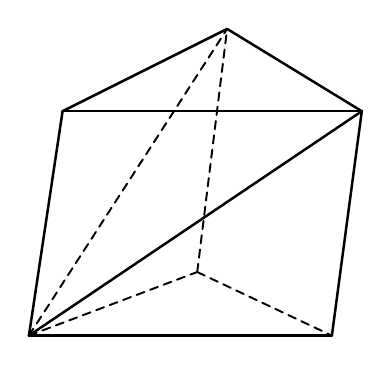
\begin{tikzpicture}[
    scale=0.95,
    line cap=round,
    line join=round,
    visible/.style={line width=0.9pt},
    hidden/.style={line width=0.7pt,dashed,dash pattern=on 3pt off 2.2pt}
]

% -------------------------------------------------
% Вершины
% Нижнее основание: A B C
% Верхнее основание: D E F
% -------------------------------------------------

\coordinate (A) at (0.20,0.20);   % нижняя левая передняя
\coordinate (B) at (2.45,1.05);   % нижняя дальняя
\coordinate (C) at (4.25,0.20);   % нижняя правая передняя

\coordinate (D) at (0.65,3.20);   % верхняя левая
\coordinate (E) at (2.85,4.30);   % верхняя вершина
\coordinate (F) at (4.65,3.20);   % верхняя правая 

% -------------------------------------------------
% Верхнее основание призмы
% -------------------------------------------------

\draw[visible] (D)--(E)--(F);
\draw[visible] (D)--(F);

% -------------------------------------------------
% Боковые рёбра призмы
% -------------------------------------------------

\draw[visible] (A)--(D);
\draw[hidden]  (B)--(E);
\draw[visible] (C)--(F);

% -------------------------------------------------
% Нижнее основание призмы
% -------------------------------------------------

\draw[visible] (A)--(C);
\draw[hidden]  (A)--(B);
\draw[hidden]  (B)--(C);

% -------------------------------------------------
% Линия сечения
% Плоскость проходит через сторону DF
% и противоположную вершину A
% -------------------------------------------------

\draw[visible] (A)--(F);
\draw[hidden] (A)--(E);
\end{tikzpicture}
}
